% ============================================================
%  PRESENTACION (Beamer) -- Algebra Lineal Aplicada
%  Pendulo invertido sobre un carro (dos configuraciones)
%  Universidad Nacional de Colombia -- Sede Medellin
%  Duracion objetivo: 20 minutos. Compilar con pdflatex/latexmk.
% ============================================================
\documentclass[aspectratio=169,11pt]{beamer}

% ── Idioma y codificacion ───────────────────────────────────
\usepackage[utf8]{inputenc}
\usepackage[T1]{fontenc}
\usepackage[spanish,es-noshorthands]{babel}

% ── Tipografia (Palatino, consistente con los informes) ─────
\usepackage{mathpazo}
\usefonttheme{serif}

% ── Matematicas, tablas, figuras ────────────────────────────
\usepackage{amsmath,amssymb,mathtools,bm}
\usepackage{booktabs}
\usepackage{array}
\usepackage{graphicx}
\usepackage{tikz}
\usetikzlibrary{arrows.meta,calc,positioning}
\usepackage[most]{tcolorbox}
\usepackage{listings}

\graphicspath{{figs/}}

% ── Paleta de colores de la presentacion ────────────────────
\definecolor{marino}{HTML}{1B4079}
\definecolor{petroleo}{HTML}{4D7C8A}
\definecolor{grisverde}{HTML}{7F9C96}
\definecolor{salvia}{HTML}{8FAD88}
\definecolor{limon}{HTML}{C7DB94}

% ── Tema Beamer: sobrio, construido sobre la paleta ─────────
\usetheme{default}
\useinnertheme{circles}
\setbeamertemplate{navigation symbols}{}
\setbeamercolor{structure}{fg=marino}
\setbeamercolor{normal text}{fg=black!85}
\setbeamercolor{alerted text}{fg=petroleo!70!black}
\setbeamercolor{frametitle}{fg=white,bg=marino}
\setbeamerfont{frametitle}{series=\bfseries,size=\large}
\setbeamercolor{section in toc}{fg=marino}
\setbeamercolor{subsection in toc}{fg=petroleo}

% Marcadores de listas: rombo en toda la presentacion
\setbeamertemplate{itemize item}{\color{marino}$\diamond$}
\setbeamertemplate{itemize subitem}{\color{petroleo}$\diamond$}

% Titulo de cada diapositiva: banda marino + filete limon
\setbeamertemplate{frametitle}{%
  \nointerlineskip
  \begin{beamercolorbox}[wd=\paperwidth,ht=2.9ex,dp=1.4ex,leftskip=1.0em]{frametitle}%
    \usebeamerfont{frametitle}\insertframetitle
  \end{beamercolorbox}%
  \nointerlineskip
  {\color{limon}\rule{\paperwidth}{1.6pt}}%
  \vskip0.4em
}

% Pie de pagina: banda clara con titulo corto, seccion y numero
\setbeamercolor{pielinea}{fg=marino,bg=limon!35}
\setbeamertemplate{footline}{%
  \begin{beamercolorbox}[wd=\paperwidth,ht=2.4ex,dp=1.1ex,leftskip=1em,rightskip=1em]{pielinea}%
    \footnotesize P\'endulo invertido sobre un carro
    \hfill \insertsectionhead
    \hfill \insertframenumber\,/\,\inserttotalframenumber
  \end{beamercolorbox}%
}

% ── Cajas para definiciones, teoremas y resultados ──────────
\newtcolorbox{cajadef}[1]{enhanced,colback=petroleo!9,colframe=petroleo!80!black,
  fonttitle=\bfseries\small,title={Definici\'on (#1)},boxrule=0.6pt,arc=1.5pt,
  left=5pt,right=5pt,top=3pt,bottom=3pt,before skip=4pt,after skip=6pt}
\newtcolorbox{cajateo}[1]{enhanced,colback=marino!7,colframe=marino,
  fonttitle=\bfseries\small,title={Teorema (#1)},boxrule=0.6pt,arc=1.5pt,
  left=5pt,right=5pt,top=3pt,bottom=3pt,before skip=4pt,after skip=6pt}
\newtcolorbox{cajares}[1]{enhanced,colback=salvia!16,colframe=salvia!55!black,
  fonttitle=\bfseries\small,title={#1},boxrule=0.6pt,arc=1.5pt,
  left=5pt,right=5pt,top=3pt,bottom=3pt,before skip=4pt,after skip=6pt}
\newtcolorbox{cajaclave}{enhanced,colback=limon!28,colframe=marino,
  boxrule=0.8pt,arc=1.5pt,left=6pt,right=6pt,top=4pt,bottom=4pt,
  before skip=4pt,after skip=6pt}

% ── Estilo de codigo ────────────────────────────────────────
\lstdefinestyle{julia}{%
  basicstyle=\ttfamily\scriptsize,
  keywordstyle=\color{marino}\bfseries,
  commentstyle=\color{grisverde!60!black}\itshape,
  stringstyle=\color{petroleo!80!black},
  showstringspaces=false,
  breaklines=true,
  columns=fullflexible,
  frame=single,
  rulecolor=\color{petroleo!60!black},
  framesep=4pt,
  xleftmargin=4pt,xrightmargin=4pt,
  aboveskip=4pt,belowskip=2pt,
  morekeywords={function,end,for,while,if,else,elseif,return,using,import,module,struct,begin,in}
}
\lstset{style=julia}

% ── Operadores y atajos ─────────────────────────────────────
\DeclareMathOperator{\rank}{rango}
\DeclareMathOperator{\Real}{Re}
\newcommand{\R}{\mathbb{R}}
\newcommand{\Cx}{\mathbb{C}}
\newcommand{\TM}{\mathrm{T}M}
\newcommand{\calC}{\mathcal{C}}
\newcommand{\calO}{\mathcal{O}}
\newcommand{\xv}{\bm{x}}
\newcommand{\uv}{\bm{u}}
\newcommand{\yv}{\bm{y}}
\newcommand{\rv}{\bm{r}}

% Franja decorativa con la paleta (para portada y cierre)
\newcommand{\franjapaleta}[1]{%
  \foreach [count=\i from 0] \c in {marino!60!white,petroleo,grisverde,salvia,limon}{%
    \fill[\c] ([xshift=\i*0.2*\paperwidth,yshift=#1]current page.south west)
      rectangle ([xshift={(\i+1)*0.2*\paperwidth},yshift={#1+0.3cm}]current page.south west);}%
}

\title{Análisis y control del péndulo invertido sobre un carro}
\author{Mateo Bedoya Rojas \and Camilo Alejandro Patiño Osorio \and Santiago Uribe Echavarría}

% ============================================================
\begin{document}

% ── Portada ─────────────────────────────────────────────────
\begin{frame}[plain]
\begin{tikzpicture}[remember picture,overlay]
  \fill[marino] (current page.south west) rectangle (current page.north east);
  \franjapaleta{1.15cm}
  \node[anchor=west, text=white, align=left]
    at ([xshift=1.1cm,yshift=1.35cm]current page.west)
    {\parbox{0.86\paperwidth}{%
      {\footnotesize\bfseries\color{limon} PROYECTO DE \'ALGEBRA LINEAL APLICADA}\\[0.8em]
      {\LARGE\bfseries An\'alisis y Control del P\'endulo Invertido\\[0.15em]
       sobre un Carro mediante \'Algebra Lineal}\\[0.9em]
      {\normalsize Espacio de estados \,\textbullet\, An\'alisis espectral \,\textbullet\,
       Realimentaci\'on de estado}\\[1.6em]
      {\footnotesize
       \begin{tabular}{@{}c@{\qquad}c@{\qquad}c@{}}
         Mateo Bedoya Rojas & Camilo Alejandro Pati\~no Osorio & Santiago Uribe Echavarr\'ia\\[0.25em]
         {\scriptsize\color{limon}{mabedoyar@unal.edu.co}} &
         {\scriptsize\color{limon}{cpatinoo@unal.edu.co}} &
         {\scriptsize\color{limon}{sauribee@unal.edu.co}}
       \end{tabular}}\\[0.5em]
      {\footnotesize\color{black!10} Facultad de Ciencias, Universidad Nacional de Colombia, Sede Medell\'in \,\textbullet\, 2026}}};
\end{tikzpicture}
\end{frame}

% ── Contenido ───────────────────────────────────────────────
\begin{frame}{Contenido}
  \tableofcontents
\end{frame}

% ============================================================
\section{El problema}
% ============================================================

\begin{frame}{El péndulo invertido sobre un carro}
  Un carro se desplaza sobre un riel horizontal; sobre \'el se articula un
  p\'endulo. El objetivo es mantenerlo en la vertical \emph{superior}
  aplicando una fuerza $u(t)$ \emph{\'unicamente sobre el carro}.
  Tres rasgos definen el reto:
  \begin{itemize}
    \item \textbf{Subactuado.} Una sola entrada debe gobernar varias variables:
          el estado vive en $\R^4$ (simple) o $\R^6$ (doble), pero $u(t)$ es un
          escalar; la matriz de entrada $B$ tiene una \'unica columna.
    \item \textbf{Inestable.} Linealizado en la vertical superior, $A$ tiene un
          eigenvalor real $\lambda>0$: cualquier desviaci\'on crece como
          $e^{\lambda t}$ y, sin control, el p\'endulo cae.
    \item \textbf{No lineal.} Las ecuaciones contienen $\sin\theta$ y
          $\cos\theta$: no son de la forma $\dot\xv=A\xv+B\uv$; hay que
          \emph{linealizar} (Taylor) alrededor del equilibrio.
  \end{itemize}
  \begin{cajaclave}
    \small Casi todas las preguntas se responden con \'algebra lineal:
    la evoluci\'on la da $e^{At}$; la estabilidad, los \emph{eigenvalores} de $A$;
    poder controlar u observar es una pregunta de \emph{rango}; y dise\~nar el
    control es \emph{reubicar eigenvalores}.
  \end{cajaclave}
\end{frame}

\begin{frame}{Dos configuraciones de complejidad creciente}
  \begin{columns}[T]
    \begin{column}{0.48\textwidth}
      \centering
      \begin{tikzpicture}[>=Stealth,thick,scale=0.8,every node/.style={transform shape}]
        \draw[gray!55] (-1.7,0) -- (3.6,0);
        \foreach \i in {-1.5,-1.1,...,3.4}{\draw[gray!45] (\i,0)--(\i-0.18,-0.2);}
        \draw[fill=petroleo!16,draw=petroleo!70!black] (0.25,0) rectangle (2.05,0.75);
        \node[petroleo!50!black] at (1.15,0.375) {\large $M$};
        \draw[fill=white,draw=petroleo!70!black] (0.6,0) circle (0.16);
        \draw[fill=white,draw=petroleo!70!black] (1.7,0) circle (0.16);
        \coordinate (P) at (1.15,0.75);
        \fill (P) circle (1.6pt);
        \coordinate (B) at ($(P)+(72:2.2)$);
        \draw[dashed,gray!70] (P) -- ++(0,2.35);
        \draw[marino,line width=1.4pt] (P) -- (B);
        \fill[marino] (B) circle (3.6pt);
        \node[right=4pt,marino] at (B) {$m,\ I$};
        \draw[->,petroleo!70!black,line width=0.9pt] (P)++(0,1.15) arc(90:72:1.15);
        \node[petroleo!70!black] at ($(P)+(81:1.62)$) {$\theta$};
        \node[right=6pt,marino] at ($(P)!0.5!(B)$) {$L$};
        \draw[->,line width=1.2pt,salvia!50!black] (-0.45,0.375)--(0.25,0.375) node[midway,above=3.5pt]{$u$};
        \draw[|-|,gray] (0.25,-0.45)--(2.05,-0.45) node[midway,below]{$x$};
      \end{tikzpicture}

      \small\textbf{Configuraci\'on I: simple.}
      Barra uniforme con momento de inercia $I$;
      $q=(x,\theta)$, estado en $\R^4$, \textbf{un} modo inestable.
    \end{column}
    \begin{column}{0.48\textwidth}
      \centering
      \begin{tikzpicture}[>=Stealth,thick,scale=0.8,every node/.style={transform shape}]
        \draw[gray!55] (-1.5,0) -- (4.0,0);
        \foreach \i in {-1.3,-0.9,...,3.8}{\draw[gray!45] (\i,0)--(\i-0.18,-0.2);}
        \draw[fill=petroleo!16,draw=petroleo!70!black] (0.5,0) rectangle (2.3,0.75);
        \node[petroleo!50!black] at (1.4,0.375) {\large $M$};
        \draw[fill=white,draw=petroleo!70!black] (0.85,0) circle (0.16);
        \draw[fill=white,draw=petroleo!70!black] (1.95,0) circle (0.16);
        \coordinate (P0) at (1.4,0.75);
        \coordinate (P1) at ($(P0)+(74:1.85)$);
        \coordinate (P2) at ($(P1)+(52:1.7)$);
        \draw[dashed,gray!70] (P0) -- ++(0,2.2);
        \draw[dashed,gray!70] (P1) -- ++(0,1.9);
        \fill (P0) circle (1.6pt);
        \draw[marino,line width=1.4pt] (P0) -- (P1);
        \draw[petroleo,line width=1.4pt] (P1) -- (P2);
        \fill[marino] (P1) circle (3.4pt);
        \fill[petroleo] (P2) circle (3.4pt);
        \node[right=4pt,marino] at (P1) {$m_1$};
        \node[right=4pt,petroleo!80!black] at (P2) {$m_2$};
        \draw[->,petroleo!70!black,line width=0.9pt] (P0)++(0,1.1) arc(90:74:1.1);
        \node[petroleo!70!black] at ($(P0)+(82:1.55)$) {$\theta_1$};
        \draw[->,petroleo!70!black,line width=0.9pt] (P1)++(0,1.25) arc(90:52:1.25);
        \node[petroleo!70!black] at ($(P1)+(69:1.52)$) {$\theta_2$};
        \node[right=3pt,marino] at ($(P0)!0.5!(P1)$) {$L_1$};
        \node[right=3pt,petroleo!80!black] at ($(P1)!0.55!(P2)$) {$L_2$};
        \draw[->,line width=1.2pt,salvia!50!black] (-0.2,0.375)--(0.5,0.375) node[midway,above=3.5pt]{$u$};
        \draw[|-|,gray] (0.5,-0.45)--(2.3,-0.45) node[midway,below]{$x$};
      \end{tikzpicture}

      \small\textbf{Configuraci\'on II: doble.}
      Masas puntuales $m_1,m_2$ y barras de masa despreciable;
      $q=(x,\theta_1,\theta_2)$, estado en $\R^6$, \textbf{dos} modos inestables.
    \end{column}
  \end{columns}
  \vspace{0.4em}
  \small El doble muestra que el mismo razonamiento algebraico \emph{escala}:
  solo crecen las matrices.
\end{frame}

% ============================================================
\section{Formalización y modelado}
% ============================================================

\begin{frame}{Coordenadas generalizadas y espacios del problema}
  Las \emph{coordenadas generalizadas} $q=(q_1,\dots,q_d)$ son un conjunto
  m\'inimo que determina la configuraci\'on; $d$ es el n\'umero de grados de libertad.
  \begin{cajadef}{Espacio de configuraci\'on}
    $M$ es el conjunto de configuraciones admisibles, parametrizado por las
    coordenadas generalizadas: una variedad diferenciable de dimensi\'on $d$.
  \end{cajadef}
  \begin{cajadef}{Espacio de estados}
    Es el \emph{fibrado tangente} $\TM$, cuyos puntos son los pares
    posici\'on--velocidad $(q,\dot q)$, de dimensi\'on $2d$.
  \end{cajadef}
  \vspace{0.2em}
  \small
  Simple: $M=\R\times S^1$, estado en $\R^4$. \quad
  Doble: $M=\R\times S^1\times S^1$, estado en $\R^6$.\\
  La din\'amica es de segundo orden: dos configuraciones iguales con velocidades
  distintas tienen futuros distintos; por eso el estado es $(q,\dot q)$.
\end{frame}

\begin{frame}{El principio variacional}
  \begin{cajadef}{Lagrangiano}
    $L:\TM\to\R$, \quad $L(q,\dot q)=T(q,\dot q)-V(q)$, con $T$ energ\'ia
    cin\'etica y $V$ energ\'ia potencial.
  \end{cajadef}
  \begin{cajadef}{Espacio de caminos y acci\'on}
    Fijados $[t_1,t_2]$ y extremos $q_a,q_b\in M$,
    \[
      \mathcal{P}=\{\gamma\in C^{\infty}([t_1,t_2],M):\gamma(t_1)=q_a,\ \gamma(t_2)=q_b\},
    \]
    \[
      S:\mathcal{P}\longrightarrow\R,\qquad
      S[\gamma]=\int_{t_1}^{t_2} L\bigl(\gamma(t),\dot\gamma(t)\bigr)\,dt .
    \]
  \end{cajadef}
  \small El principio de Hamilton: las trayectorias f\'isicas hacen
  \emph{estacionaria} la acci\'on ($\delta S=0$); son los puntos cr\'iticos del
  funcional $S$ en un espacio de dimensi\'on infinita.
\end{frame}

\begin{frame}{Ecuaciones de Euler--Lagrange}
  \begin{cajateo}{Ecuaciones de Euler--Lagrange}
    $\gamma$ es punto cr\'itico de la acci\'on si y solo si, para cada
    $i=1,\dots,d$,
    \[
      \frac{d}{dt}\!\left(\frac{\partial L}{\partial \dot q_i}\right)
      -\frac{\partial L}{\partial q_i}=Q_i ,
    \]
    con $Q_i$ la fuerza generalizada no conservativa (control $u$, fricci\'on $-b\dot x$).
  \end{cajateo}
  \vspace{0.3em}
  \textbf{Plan de trabajo} (id\'entico para ambas configuraciones):
  \begin{enumerate}
    \small
    \item[$i$.] elegir las coordenadas generalizadas $q$;
    \item[$ii$.] escribir las posiciones de cada masa y derivarlas para obtener
                 las velocidades;
    \item[$iii$.] formar $T$ y $V$, y con ellas $L=T-V$;
    \item[$iv$.] aplicar Euler--Lagrange para obtener las ecuaciones no lineales;
    \item[$v$.] linealizar y reescribir en el espacio de estados.
  \end{enumerate}
\end{frame}

\begin{frame}{Configuración I: modelo no lineal}
  Con $q=(x,\theta)$, $\theta$ medido desde la vertical superior:
  \[
    T=\tfrac12 M\dot x^2
     +\tfrac12 m\bigl(\dot x^2+2L\dot x\dot\theta\cos\theta+L^2\dot\theta^2\bigr)
     +\tfrac12 I\dot\theta^2,
    \qquad V=mgL\cos\theta .
  \]
  Euler--Lagrange con $Q_x=u-b\dot x$, $Q_\theta=0$, agrupado en la
  \emph{ecuaci\'on del manipulador}:
  \[
    \mathbf{M}(q)\,\ddot q+\mathbf{C}(q,\dot q)\,\dot q+\mathbf{G}(q)=\bm F u,
    \qquad \bm F=(1,0)^\top,
  \]
  \vspace{-0.9em}
  \[
  {\footnotesize
  \mathbf{M}(q)=\begin{pmatrix} M{+}m & mL\cos\theta\\ mL\cos\theta & I{+}mL^2\end{pmatrix},\quad
  \mathbf{C}(q,\dot q)=\begin{pmatrix} b & -mL\dot\theta\sin\theta\\ 0 & 0\end{pmatrix},\quad
  \mathbf{G}(q)=\begin{pmatrix} 0\\ -mgL\sin\theta\end{pmatrix},}
  \]
  \vspace{-0.4em}
  \begin{itemize}
    \small
    \item $\mathbf{M}(q)$: \emph{matriz de masa}; \
          $\mathbf{C}(q,\dot q)\,\dot q$: t\'ermino centr\'ifugo y fricci\'on
          $b\dot x$; \ $\mathbf{G}(q)$: gravedad.
    \item Como en el doble, $\mathbf{M}(q)$ es sim\'etrica y definida positiva;
          su determinante en $\theta=0$ es el $D_0$ de la linealizaci\'on.
  \end{itemize}
  \begin{cajaclave}
    \small \textbf{La firma de la inestabilidad:} el t\'ermino $-mgL\sin\theta$
    de $\mathbf{G}(q)$ produce, al linealizar, un coeficiente \emph{positivo} y
    con \'el un eigenvalor real positivo. Entre ``colgar'' y ``estar invertido''
    hay, literalmente, un signo.
  \end{cajaclave}
\end{frame}

\begin{frame}{Configuración II: forma matricial de la mecánica}
  Con $q=(x,\theta_1,\theta_2)$ y masas puntuales $m_1,m_2$, las ecuaciones de
  Euler--Lagrange se agrupan en la \emph{ecuaci\'on del manipulador}, la forma
  est\'andar de la mec\'anica lagrangiana:
  \[
    \mathbf{M}(q)\,\ddot q+\mathbf{C}(q,\dot q)\,\dot q+\mathbf{G}(q)=\bm{F}u,
    \qquad \bm F=(1,0,0)^\top,
  \]
  \[
  {\footnotesize
  \mathbf{M}(q)=\!\begin{pmatrix}
   M{+}m_1{+}m_2 & L_1(m_1{+}m_2)c_1 & L_2 m_2 c_2\\
   L_1(m_1{+}m_2)c_1 & L_1^2(m_1{+}m_2) & L_1L_2 m_2 c_{12}\\
   L_2 m_2 c_2 & L_1L_2 m_2 c_{12} & L_2^2 m_2
  \end{pmatrix},
  \quad
  \mathbf{G}(q)=\begin{pmatrix} 0\\ -(m_1{+}m_2)gL_1\sin\theta_1\\ -m_2 gL_2\sin\theta_2\end{pmatrix},}
  \]
  con $c_1=\cos\theta_1$, $c_2=\cos\theta_2$, $c_{12}=\cos(\theta_1{-}\theta_2)$.
  \vspace{0.3em}
  \begin{itemize}
    \small
    \item Las aceleraciones $\ddot q$ entran \emph{linealmente}: $\mathbf{M}(q)$
          es la \emph{matriz de masa}, $\mathbf{C}(q,\dot q)\,\dot q$ agrupa los
          t\'erminos centr\'ifugos y de Coriolis, y $\mathbf{G}(q)$ la gravedad.
    \item Verificaci\'on por reducci\'on: con $m_2=0$ (y $I=b=0$ en el simple)
          ambas derivaciones coinciden.
  \end{itemize}
\end{frame}

\begin{frame}[fragile]{De $\mathbf{M}(q)\,\ddot q=\mathrm{rhs}$ a las aceleraciones}
  Escribir $\mathbf{M}(q)\,\ddot q=\mathrm{rhs}$ \textbf{no} es una
  factorizaci\'on: es \emph{despejar}. Como $\ddot q$ entra linealmente, se pasan
  al lado derecho (\emph{right-hand side}) todos los t\'erminos que no contienen
  aceleraciones:
  \[
    \mathbf{M}(q)\,\ddot q
    =\underbrace{\bm F u-\mathbf{C}(q,\dot q)\,\dot q-\mathbf{G}(q)}_{=:\ \mathrm{rhs}(q,\,\dot q,\,u)} .
  \]
  \begin{columns}[T]
    \begin{column}{0.56\textwidth}
\begin{lstlisting}
Mq  = [ M+m1+m2       (m1+m2)*L1*c1  m2*L2*c2;
        (m1+m2)*L1*c1 (m1+m2)*L1^2   m2*L1*L2*c12;
        m2*L2*c2      m2*L1*L2*c12   m2*L2^2 ]
rhs = [ F + (m1+m2)*L1*s1*w1^2 + m2*L2*s2*w2^2,
        (m1+m2)*g*L1*s1 - m2*L1*L2*s12*w2^2,
        m2*g*L2*s2 + m2*L1*L2*s12*w1^2 ]
qdd = cholesky(Symmetric(Mq)) \ rhs
\end{lstlisting}
    \end{column}
    \begin{column}{0.42\textwidth}
      \small
      $\mathbf{M}(q)$ es sim\'etrica y \emph{definida positiva}
      $\Rightarrow$ invertible: $\ddot q$ existe y es \'unico.
      \vspace{0.4em}

      La factorizaci\'on aparece al \emph{resolver}:
      \texttt{cholesky(Symmetric(Mq))} factoriza $\mathbf{M}=LL^\top$
      ---la \textbf{factorizaci\'on de Cholesky}, que existe exactamente para
      matrices sim\'etricas definidas positivas--- y
      \texttt{\textbackslash} resuelve dos sistemas triangulares, sin calcular
      $\mathbf{M}^{-1}$.
    \end{column}
  \end{columns}
\end{frame}

\begin{frame}{Linealización: Taylor de primer orden}
  Escribimos el sistema como $\dot\xv=f(\xv,u)$ con equilibrio
  $f(\xv^\star,0)=\bm 0$ y truncamos el desarrollo de Taylor:
  \[
    A=\left.\frac{\partial f}{\partial \xv}\right|_{(\xv^\star,0)}\in\R^{n\times n},
    \qquad
    B=\left.\frac{\partial f}{\partial u}\right|_{(\xv^\star,0)}\in\R^{n\times m},
    \qquad
    \sin\theta\approx\theta,\quad\cos\theta\approx 1 .
  \]
  \begin{cajares}{Hip\'otesis (desviaciones peque\~nas)}
    El sistema opera en una vecindad del equilibrio erguido: los t\'erminos de
    segundo orden ($\theta^2$, $\dot\theta^2\theta$, $\dot x\dot\theta$, \dots)
    se desprecian.
  \end{cajares}
  \small El modelo lineal es fiel \emph{localmente}; pero ese es justamente el
  r\'egimen en que opera un controlador estabilizante: una vez erguido, el
  p\'endulo permanece cerca de $\theta=0$.
\end{frame}

\begin{frame}{Representación en espacio de estados}
  \begin{cajadef}{Representaci\'on en espacio de estados}
    Un sistema lineal de tiempo continuo se escribe como
    \[
      \dot\xv=A\xv+B\uv,\qquad \yv=C\xv+D\uv,
    \]
    con estado $\xv\in\R^n$, entrada $\uv\in\R^m$ y salida $\yv\in\R^p$.
  \end{cajadef}
  Cada matriz tiene nombre y papel propios:
  \begin{itemize}
    \small
    \item $A\in\R^{n\times n}$ --- \textbf{matriz de din\'amica}: la
          transformaci\'on lineal que rige la evoluci\'on de las desviaciones;
          $\dot\xv=A\xv$ es la forma vectorial de $n$ EDO de primer orden
          acopladas.
    \item $B\in\R^{n\times m}$ --- \textbf{matriz de entrada}: c\'omo entra la
          fuerza de control en el sistema.
    \item $C\in\R^{p\times n}$ --- \textbf{matriz de salida}: selecciona qu\'e
          se mide con los sensores.
    \item $D\in\R^{p\times m}$ --- \textbf{matriz de transmisi\'on directa}:
          efecto instant\'aneo de la entrada sobre la salida; en nuestro sistema
          $D=\bm 0$, pues la fuerza no aparece en las mediciones.
  \end{itemize}
\end{frame}

\begin{frame}{Espacio de estados: péndulo simple}
  Estado $\xv=(x,\dot x,\theta,\dot\theta)^\top\in\R^4$; con
  $D_0=(M{+}m)(I{+}mL^2)-(mL)^2>0$, la linealizaci\'on da
  \[
  {\footnotesize
  A=\begin{pmatrix}
  0&1&0&0\\
  0&-\dfrac{b(I{+}mL^2)}{D_0}&-\dfrac{m^2gL^2}{D_0}&0\\[6pt]
  0&0&0&1\\
  0&\dfrac{bmL}{D_0}&\dfrac{(M{+}m)mgL}{D_0}&0
  \end{pmatrix},\quad
  B=\begin{pmatrix}0\\[2pt]\dfrac{I{+}mL^2}{D_0}\\[6pt]0\\[2pt]-\dfrac{mL}{D_0}\end{pmatrix},\quad
  C=\begin{pmatrix}1&0&0&0\\0&0&1&0\end{pmatrix},\quad D=\bm 0.}
  \]
  \begin{itemize}
    \small
    \item $C$ mide posici\'on del carro y \'angulo ($p=2$): las velocidades
          \emph{no} se miden.
    \item El signo \emph{positivo} de $A_{4,3}=(M{+}m)mgL/D_0$ es la firma
          algebraica de la inestabilidad: producir\'a un eigenvalor real
          positivo.
  \end{itemize}
\end{frame}

\begin{frame}{Espacio de estados: péndulo doble}
  Estado $\xv=(x,\dot x,\theta_1,\dot\theta_1,\theta_2,\dot\theta_2)^\top\in\R^6$;
  linealizando alrededor de $\theta_1=\theta_2=0$:
  \[
  {\footnotesize
  A=\begin{pmatrix}
  0&1&0&0&0&0\\
  0&0&-\dfrac{g(m_1{+}m_2)}{M}&0&0&0\\[4pt]
  0&0&0&1&0&0\\
  0&0&\dfrac{g(M{+}m_1)(m_1{+}m_2)}{ML_1 m_1}&0&-\dfrac{g m_2}{L_1 m_1}&0\\[4pt]
  0&0&0&0&0&1\\
  0&0&-\dfrac{g(m_1{+}m_2)}{L_2 m_1}&0&\dfrac{g(m_1{+}m_2)}{L_2 m_1}&0
  \end{pmatrix},}
  \]
  \vspace{-0.5em}
  \[
  {\footnotesize
  B=\Bigl(0,\ \tfrac1M,\ 0,\ -\tfrac{1}{ML_1},\ 0,\ 0\Bigr)^{\!\top},\qquad
  C=\begin{pmatrix}1&0&0&0&0&0\\0&0&1&0&0&0\\0&0&0&0&1&0\end{pmatrix},\qquad
  D=\bm 0.}
  \]
  \vspace{-0.3em}
  \begin{itemize}
    \small
    \item $C$ mide $x,\theta_1,\theta_2$ ($p=3$); los coeficientes gravitatorios
          positivos $A_{4,3}$ y $A_{6,5}$ anticipan \emph{dos} modos inestables.
    \item Verificaci\'on por reducci\'on: con $m_2=0$ (y $I=b=0$ en el simple)
          el doble se reduce al simple.
  \end{itemize}
\end{frame}

% ============================================================
\section{Herramientas de álgebra lineal}
% ============================================================

\begin{frame}{La exponencial matricial y la solución del sistema}
  \begin{cajadef}{Exponencial matricial}
    $\displaystyle e^{At}=\sum_{k=0}^{\infty}\frac{(At)^k}{k!}$, serie
    convergente para todo $t$ y toda $A\in\R^{n\times n}$.
  \end{cajadef}
  \begin{cajateo}{Soluci\'on del sistema lineal}
    La soluci\'on de $\dot\xv=A\xv+B\uv$ con $\xv(0)=\xv_0$ es
    \[
      \xv(t)=e^{At}\xv_0+\int_0^t e^{A(t-s)}B\,\uv(s)\,ds .
    \]
  \end{cajateo}
  Si $A=P\Lambda P^{-1}$ es diagonalizable:
  $e^{At}=P\,\mathrm{diag}(e^{\lambda_1 t},\dots,e^{\lambda_n t})\,P^{-1}$.
  \begin{cajaclave}
    \small $\xv(t)\to\bm 0$ cuando $t\to\infty$ \emph{si y solo si}
    $\Real(\lambda_i)<0$ para todo eigenvalor de $A$.
  \end{cajaclave}
\end{frame}

\begin{frame}{Eigenvalores y polinomio característico}
  \begin{cajadef}{Polinomio caracter\'istico y espectro}
    $p(\lambda)=\det(A-\lambda I)$, de grado $n$; sus ra\'ices son los
    eigenvalores y su conjunto es el espectro $\sigma(A)$.
  \end{cajadef}
  \textbf{Ejemplo (bloque angular del simple, $b=0$):} con
  $\kappa=(M{+}m)mgL/D_0>0$,
  \[
    A_\theta=\begin{pmatrix}0&1\\\kappa&0\end{pmatrix},
    \qquad
    p(\lambda)=\lambda^2-\kappa
    \quad\Longrightarrow\quad
    \lambda=\pm\sqrt{\kappa}.
  \]
  \small Un eigenvalor \emph{real positivo}: el equilibrio es inestable. Con los
  par\'ametros del informe $\sqrt{\kappa}\approx 4.22$, muy pr\'oximo al
  eigenvalor $+4.21$ del sistema completo (la peque\~na diferencia la introducen
  la fricci\'on y el acoplamiento).
\end{frame}

\begin{frame}{El teorema de Cayley--Hamilton}
  \begin{cajateo}{Cayley--Hamilton}
    Toda matriz cuadrada satisface su propio polinomio caracter\'istico:
    si $p(\lambda)=\lambda^n+c_{n-1}\lambda^{n-1}+\cdots+c_0$, entonces
    \[
      p(A)=A^n+c_{n-1}A^{n-1}+\cdots+c_1A+c_0I=0 .
    \]
  \end{cajateo}
  Consecuencia:
  \[
    A^n=-\bigl(c_{n-1}A^{n-1}+\cdots+c_1A+c_0I\bigr),
  \]
  y por inducci\'on toda potencia $A^{n+j}$ es combinaci\'on lineal de
  $I,A,\dots,A^{n-1}$.
  \begin{cajaclave}
    \small Las potencias ``altas'' de $A$ no aportan nada nuevo. Esta es la
    raz\'on de fondo de que las matrices de controlabilidad y observabilidad
    solo necesiten potencias hasta $A^{n-1}$.
  \end{cajaclave}
\end{frame}

\begin{frame}{Polinomio minimal y descomposición primaria}
  \begin{cajadef}{Polinomio minimal}
    Para $T:V\to V$, $m(\lambda)$ es el polinomio m\'onico de grado m\'inimo con
    $m(T)=0$. Divide a todo polinomio que anule a $T$ y sus ra\'ices son
    exactamente los eigenvalores.
  \end{cajadef}
  \begin{cajateo}{Descomposici\'on primaria}
    Si $m(\lambda)=\prod_{i=1}^{k}p_i(\lambda)$ con los $p_i$ coprimos dos a
    dos, el espacio se descompone en suma directa de subespacios
    $T$-invariantes:
    \[
      V=\bigoplus_{i=1}^{k}\mathrm{N}\!\bigl(p_i(T)\bigr).
    \]
  \end{cajateo}
\end{frame}

\begin{frame}{Forma de Jordan: nuestro sistema la ejercita}
  \begin{cajares}{Corolario (diagonalizaci\'on y Jordan)}
    Sobre $\Cx$, $m(\lambda)=\prod_i(\lambda-\alpha_i)^{d_i}$. Si todos los
    $d_i=1$, $T$ es \emph{diagonalizable} (base de eigenvectores). Los factores
    con $d_i>1$ dan los bloques de la \emph{forma can\'onica de Jordan}.
  \end{cajares}
  \begin{itemize}
    \small
    \item Lazo cerrado (ambas configuraciones) y lazo abierto del \emph{simple}:
          eigenvalores distintos $\Rightarrow$ diagonalizables.
    \item Lazo abierto del \emph{doble}: $\lambda=0$ con multiplicidad
          algebraica 2 y geom\'etrica 1 $\Rightarrow$ \emph{defectuosa}. El bloque
          responsable es el doble integrador del carro,
          $\bigl(\begin{smallmatrix}0&1\\0&0\end{smallmatrix}\bigr)$:
          su exponencial arrastra el t\'ermino secular $t$, que es la deriva del
          carro a velocidad constante.
    \item La fricci\'on del simple ($b\neq0$) parte ese bloque en
          $\{0,\,-0.077\}$: por eso su $A$ s\'i es diagonalizable.
  \end{itemize}
\end{frame}

\begin{frame}{Estabilidad: Hurwitz y Lyapunov}
  \begin{cajadef}{Estabilidad asint\'otica y matriz de Hurwitz}
    $\xv=\bm 0$ es asint\'oticamente estable si toda trayectoria tiende a
    $\bm 0$. $A$ es \emph{de Hurwitz} si $\Real(\lambda_i)<0$ para todo
    eigenvalor.
  \end{cajadef}
  \begin{cajateo}{Criterio espectral}
    $\bm 0$ es asint\'oticamente estable si y solo si $A$ es de Hurwitz.
  \end{cajateo}
  \begin{cajateo}{Lyapunov para sistemas lineales}
    $A$ es de Hurwitz si y solo si, dada cualquier $Q\succ0$ sim\'etrica, la
    ecuaci\'on $A^\top P+PA=-Q$ tiene una \'unica soluci\'on sim\'etrica
    $P\succ0$.
  \end{cajateo}
\end{frame}

\begin{frame}{Controlabilidad: el criterio de rango de Kalman}
  \begin{cajadef}{Controlabilidad}
    $(A,B)$ es completamente controlable si para cualesquiera $\xv_0,\xv_f$
    existe $T>0$ y una entrada $\uv:[0,T]\to\R^m$ que lleva de $\xv_0$ a $\xv_f$.
  \end{cajadef}
  \begin{cajadef}{Matriz de controlabilidad}
    $\calC=\begin{pmatrix}B & AB & A^2B & \cdots & A^{n-1}B\end{pmatrix}\in\R^{n\times nm}$
    \ (Cayley--Hamilton justifica truncar en $A^{n-1}B$).
  \end{cajadef}
  \begin{cajateo}{Criterio de rango de Kalman}
    $(A,B)$ es completamente controlable si y solo si $\rank(\calC)=n$.
  \end{cajateo}
  \small\textbf{Test PBH:} equivalentemente,
  $\rank[\,A-\lambda I \mid B\,]=n$ para todo $\lambda\in\Cx$; falla en
  $\lambda_i$ justo cuando un eigenvector izquierdo es ortogonal a $B$: un modo
  que la entrada ``no toca''.
\end{frame}

\begin{frame}{Observabilidad y dualidad}
  Medimos solo $\yv=C\xv$ (posici\'on y \'angulos, no velocidades):
  ?`basta para reconstruir el estado?
  \begin{cajadef}{Observabilidad y matriz de observabilidad}
    $(C,A)$ es completamente observable si $\xv_0$ queda determinado por
    $\yv(t)$ y $\uv(t)$ en un intervalo finito;
    $\calO=\bigl(C;\ CA;\ \dots;\ CA^{n-1}\bigr)\in\R^{np\times n}$.
  \end{cajadef}
  \begin{cajateo}{Criterio de observabilidad}
    $(C,A)$ es completamente observable si y solo si $\rank(\calO)=n$.
  \end{cajateo}
  \begin{cajateo}{Dualidad}
    $(A,B)$ controlable $\iff$ $(B^\top,A^\top)$ observable; \quad
    $(C,A)$ observable $\iff$ $(A^\top,C^\top)$ controlable.
  \end{cajateo}
  \small Aqu\'i $\rank(\calO)=n$: las mediciones bastan para reconstruir las velocidades.
\end{frame}

% ============================================================
\section{Diseño de controladores}
% ============================================================

\begin{frame}{Realimentación de estado y asignación de polos}
  Ley de control $\uv=-K\xv$: la din\'amica pasa a ser
  $\dot\xv=(A-BK)\xv$, estable si y solo si $A-BK$ es de Hurwitz.
  \begin{cajateo}{Asignaci\'on arbitraria de polos}
    Si $(A,B)$ es completamente controlable, para cualquier conjunto
    $\{\mu_1,\dots,\mu_n\}\subset\Cx$ cerrado bajo conjugaci\'on existe $K$ con
    $\sigma(A-BK)=\{\mu_1,\dots,\mu_n\}$. Para $m=1$, $K$ es \'unica.
  \end{cajateo}
  \begin{cajares}{Proposici\'on (F\'ormula de Ackermann)}
    Para una entrada, con polinomio deseado
    $p_d(\lambda)=\prod_{i=1}^{n}(\lambda-\mu_i)$:
    \[
      K=\bm e_n^\top\,\calC^{-1}\,p_d(A),
      \qquad \bm e_n^\top=(0,\dots,0,1).
    \]
  \end{cajares}
  \small Requiere $\calC$ invertible (controlabilidad) y usa Cayley--Hamilton:
  $p_d(A)$ es una suma finita de potencias. Exige \emph{elegir} los polos a mano.
\end{frame}

\begin{frame}{Control óptimo: el regulador lineal cuadrático}
  \begin{cajadef}{Problema LQR}
    Dadas $Q\succeq0$ (penaliza desviaciones) y $R\succ0$ (penaliza esfuerzo),
    minimizar
    \[
      J=\int_0^{\infty}\bigl(\xv^\top Q\,\xv+\uv^\top R\,\uv\bigr)\,dt .
    \]
  \end{cajadef}
  \begin{cajateo}{Soluci\'on del LQR}
    Si $(A,B)$ es controlable, el \'optimo es $\uv=-K\xv$ con
    $K=R^{-1}B^\top P$, donde $P\succ0$ es la soluci\'on estabilizante de la
    ecuaci\'on algebraica de Riccati (CARE)
    \[
      A^\top P+PA-PBR^{-1}B^\top P+Q=0 .
    \]
    El lazo cerrado $A-BK$ resulta autom\'aticamente de Hurwitz.
  \end{cajateo}
  \small Frente a Ackermann: una elecci\'on de pesos $(Q,R)$ da polos \'optimos y escala a $n=6$.
\end{frame}

\begin{frame}{Resolver la Riccati: la matriz hamiltoniana}
  La \textbf{CARE} (\emph{Continuous-time Algebraic Riccati Equation}: la
  ecuaci\'on algebraica de Riccati de tiempo continuo) es \emph{cuadr\'atica}
  en $P$; su soluci\'on se reduce a eigenvalores y subespacios invariantes:
  \[
    H=\begin{pmatrix}A & -BR^{-1}B^\top\\ -Q & -A^\top\end{pmatrix}\in\R^{2n\times2n}.
  \]
  \vspace{-0.5em}
  \begin{enumerate}
    \small
    \item[$i$.] Calcular eigenvalores y eigenvectores de $H$.
    \item[$ii$.] Seleccionar los $n$ asociados a $\Real(\lambda)<0$
          (el \emph{subespacio invariante estable}).
    \item[$iii$.] Partir esos eigenvectores en bloques $V_1,V_2\in\R^{n\times n}$
          y formar $P=V_2V_1^{-1}$.
  \end{enumerate}
  \begin{cajaclave}
    \footnotesize \textbf{?`Por qu\'e hay exactamente $n$ estables?} Como
    $\xv^\top Q\,\xv=\lVert Q^{1/2}\xv\rVert^2$, donde $Q^{1/2}$ es la ra\'iz
    cuadrada de $Q$ ($Q^{1/2}Q^{1/2}=Q$; aqu\'i,
    $\mathrm{diag}(\sqrt{q_{ii}})$), el costo mide el estado a trav\'es de la salida
    ficticia $\bm z=Q^{1/2}\xv$. En nuestro caso $(A,B)$ es \emph{controlable} y
    $(Q^{1/2},A)$ es \emph{observable} ---ambos verificados con el criterio de
    rango de Kalman---: ning\'un modo inestable escapa del control ni se oculta
    del costo, y $H$ tiene exactamente $n$ eigenvalores estables y ninguno sobre
    el eje imaginario.
  \end{cajaclave}
\end{frame}

\begin{frame}[fragile]{Los dos pseudocódigos centrales}
  \begin{columns}[T]
    \begin{column}{0.52\textwidth}
      \small\textbf{LQR: Riccati v\'ia hamiltoniana}
\begin{lstlisting}
function solve_care(A, B, Q, R)
    n = size(A, 1)
    S = B * inv(R) * B'
    H = [A -S; -Q -A']     # 2n x 2n
    eig = eigen(H)
    est = findall(real.(eig.values) .< 0)
    V  = eig.vectors[:, est]
    V1 = V[1:n, :]; V2 = V[n+1:2n, :]
    P  = real.(V2 / V1)    # P = V2 V1^-1
    return (P + P') / 2    # simetrizar
end
K = inv(R) * B' * P        # ganancia
\end{lstlisting}
    \end{column}
    \begin{column}{0.46\textwidth}
      \small\textbf{Asignaci\'on de polos: Ackermann}
\begin{lstlisting}
function ackermann(A, B, polos)
    n = size(A, 1)
    C = hcat([A^k * B for k in 0:n-1]...)
    @assert rank(C) == n    # Kalman
    phiA = prod(A - p * I for p in polos)
    en = [zeros(1, n-1) 1.0]  # e_n'
    return en * inv(C) * phiA
end
\end{lstlisting}
      \vspace{0.2em}
      \scriptsize Cada l\'inea es un concepto del curso: matriz de
      controlabilidad, criterio de rango, Cayley--Hamilton, subespacio
      invariante estable.
    \end{column}
  \end{columns}
\end{frame}

% ============================================================
\section{Implementación y resultados}
% ============================================================

\begin{frame}{Arquitectura del código (Julia)}
  \centering
  \begin{tikzpicture}[>=Stealth, node distance=0.3cm,
      caja/.style={draw=marino!70, rounded corners=2pt, align=center,
                   font=\footnotesize, minimum height=1.05cm, inner sep=5pt}]
    \node[caja, fill=marino!12] (model) {\texttt{model\_*.jl}\\ f\'isica no lineal};
    \node[caja, fill=petroleo!14, right=of model] (lin) {\texttt{linearization.jl}\\ $A,B,C,D$ + espectro + Kalman};
    \node[caja, fill=grisverde!20, right=of lin] (ctrl) {\texttt{controller.jl}\\ LQR y Ackermann};
    \node[caja, fill=salvia!25, right=of ctrl] (sim) {simulaci\'on\\ no lineal};
    \draw[->, thick, marino] (model) -- (lin);
    \draw[->, thick, marino] (lin) -- (ctrl);
    \draw[->, thick, marino] (ctrl) -- (sim);
  \end{tikzpicture}
  \vspace{0.6em}
  \begin{itemize}
    \small
    \item La \emph{f\'isica} (un m\'odulo por configuraci\'on) est\'a separada de
          los \emph{algoritmos}, gen\'ericos en la dimensi\'on: el mismo c\'odigo
          analiza $\R^4$ y $\R^6$.
    \item Los valores y figuras se \emph{generan} corriendo
          \texttt{main\_simple.jl} y \texttt{main\_double.jl}; nada se transcribe.
    \item Verificaci\'on: el Jacobiano anal\'itico coincide con el num\'erico
          hasta $\sim10^{-11}$; dos cuadernos Pluto permiten variar par\'ametros
          y pesos en vivo.
  \end{itemize}
\end{frame}

\begin{frame}{Lazo abierto: espectros, rangos y lazo cerrado}
  \begin{columns}[T]
    \begin{column}{0.44\textwidth}
      \small
      \begin{tabular}{@{}lll@{}}
        \toprule
        \textbf{Config.} & $\sigma(A)$ & \textbf{Diagn\'ostico}\\
        \midrule
        Simple & $+4.21,\ 0,$ & inestable\\
        ($n=4$) & $-0.077,\ -4.23$ & (1 modo)\\[2pt]
        Doble & $\pm8.57,\ \pm4.09,$ & inestable\\
        ($n=6$) & $0,\ 0$ & (2 modos)\\
        \bottomrule
      \end{tabular}
      \vspace{0.6em}

      En ambos casos
      \[
        \rank(\calC)=n, \qquad \rank(\calO)=n :
      \]
      completamente controlables y observables; el espectro \emph{puede}
      reubicarse.
    \end{column}
    \begin{column}{0.54\textwidth}
      \centering
      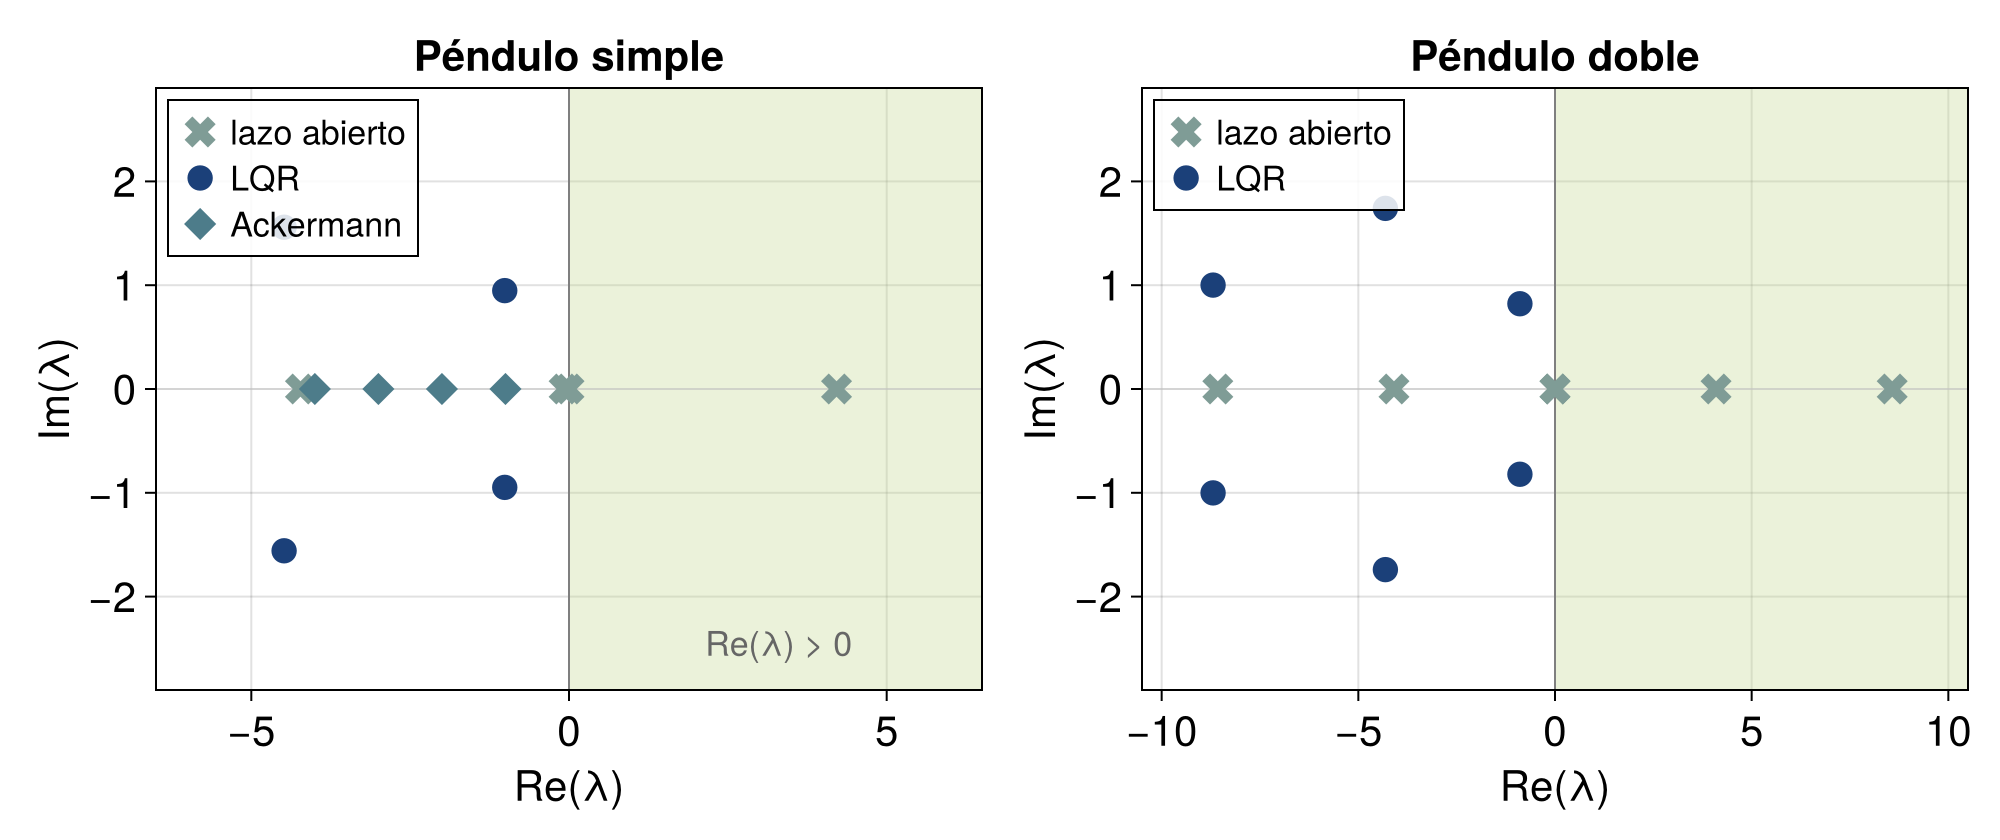
\includegraphics[width=\linewidth]{slides_polos.png}

      {\scriptsize La realimentaci\'on $\uv=-K\xv$ arrastra todo el espectro al
       semiplano izquierdo.}
    \end{column}
  \end{columns}
\end{frame}

\begin{frame}{Ganancias y polos de lazo cerrado}
  \small
  \begin{center}
  \renewcommand{\arraystretch}{1.25}
  \begin{tabular}{@{}>{\raggedright\arraybackslash}p{0.30\linewidth}p{0.62\linewidth}@{}}
    \toprule
    \textbf{M\'etodo} & \textbf{Ganancia $K$ y polos de lazo cerrado}\\
    \midrule
    Simple --- LQR\newline $Q=\mathrm{diag}(1,0,10,0)$, $R=0.1$ &
      $K=(-3.16,\,-4.69,\,-45.39,\,-10.93)$\newline
      $\sigma=\{-4.48\pm1.56i,\ -1.01\pm0.95i\}$\\
    Simple --- Ackermann\newline (polos $\{-1,-2,-3,-4\}$) &
      $K=(-1.75,\,-3.75,\,-39.01,\,-9.60)$\newline
      $\sigma=\{-1,\,-2,\,-3,\,-4\}$\\
    Doble --- LQR\newline $Q=\mathrm{diag}(1,0,10,0,10,0)$, $R=0.1$ &
      $K=(3.16,\,5.82,\,-191.55,\,-10.99,\,228.32,\,36.14)$\newline
      $\sigma=\{-8.69\pm1.00i,\ -4.31\pm1.74i,\ -0.89\pm0.82i\}$\\
    \bottomrule
  \end{tabular}
  \end{center}
  \vspace{0.2em}
  Las ganancias mucho mayores del doble reflejan sus \emph{dos} modos
  inestables, uno de ellos r\'apido ($\lambda=+8.57$).
\end{frame}

\begin{frame}{Respuesta del péndulo simple ($\theta_0=0.15$ rad)}
  \centering
  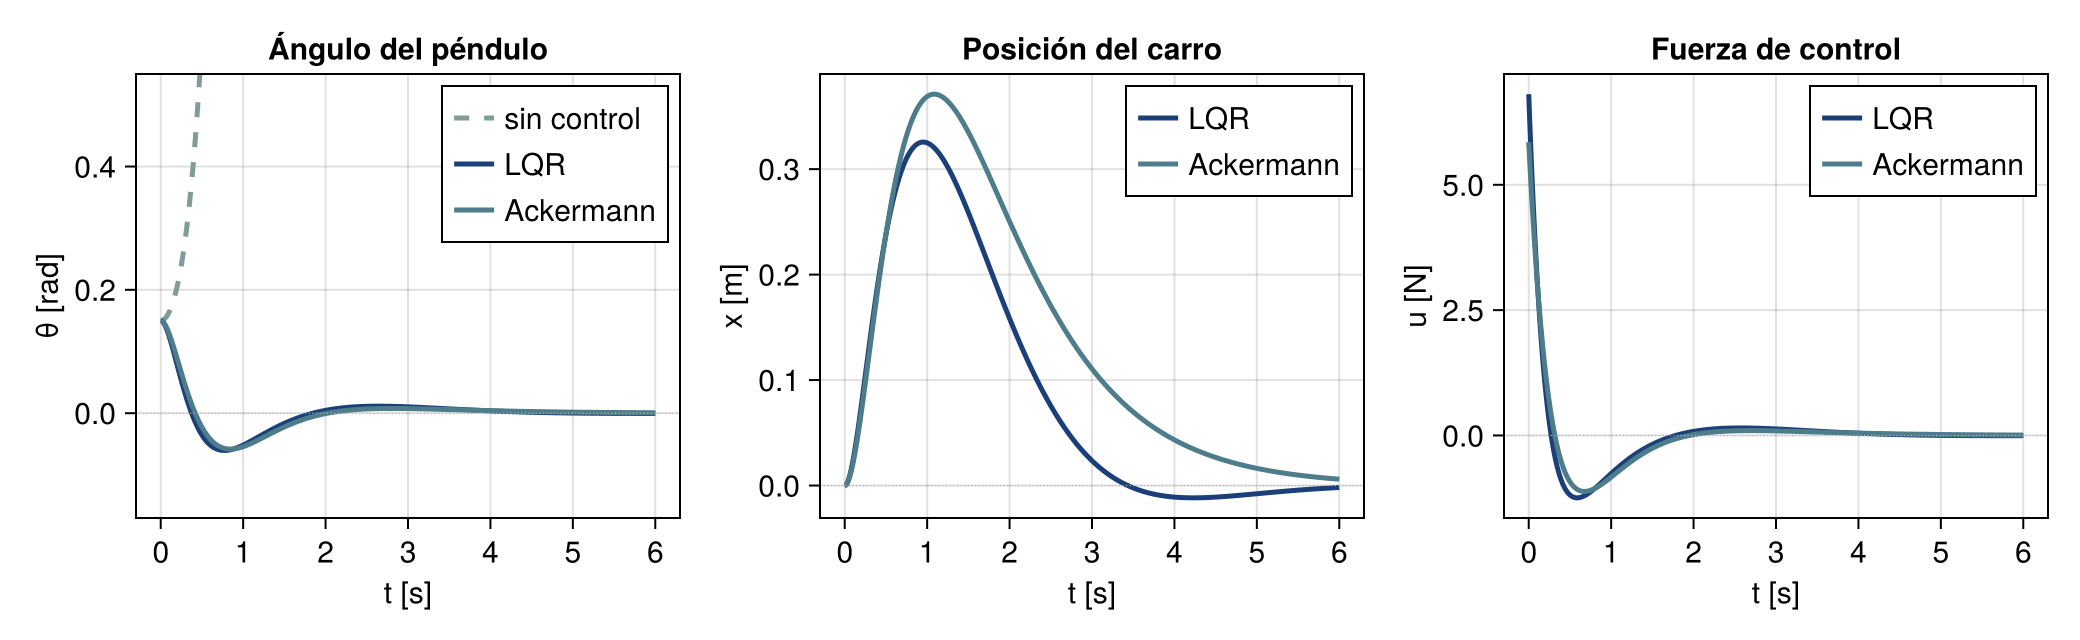
\includegraphics[width=0.98\linewidth]{slides_simple_respuesta.png}
  \vspace{0.2em}

  \small Verificaci\'on sobre el modelo \emph{no lineal}: sin control el
  \'angulo diverge; con LQR, $t_s\approx1.45$ s y $\max|u|=6.8$ N; con
  Ackermann, $t_s\approx1.54$ s y $\max|u|=5.9$ N
  (umbral $|\theta|<0.02$ rad $\approx1.1^\circ$).
\end{frame}

\begin{frame}{Distintos casos: robustez frente a la condición inicial}
  \centering
  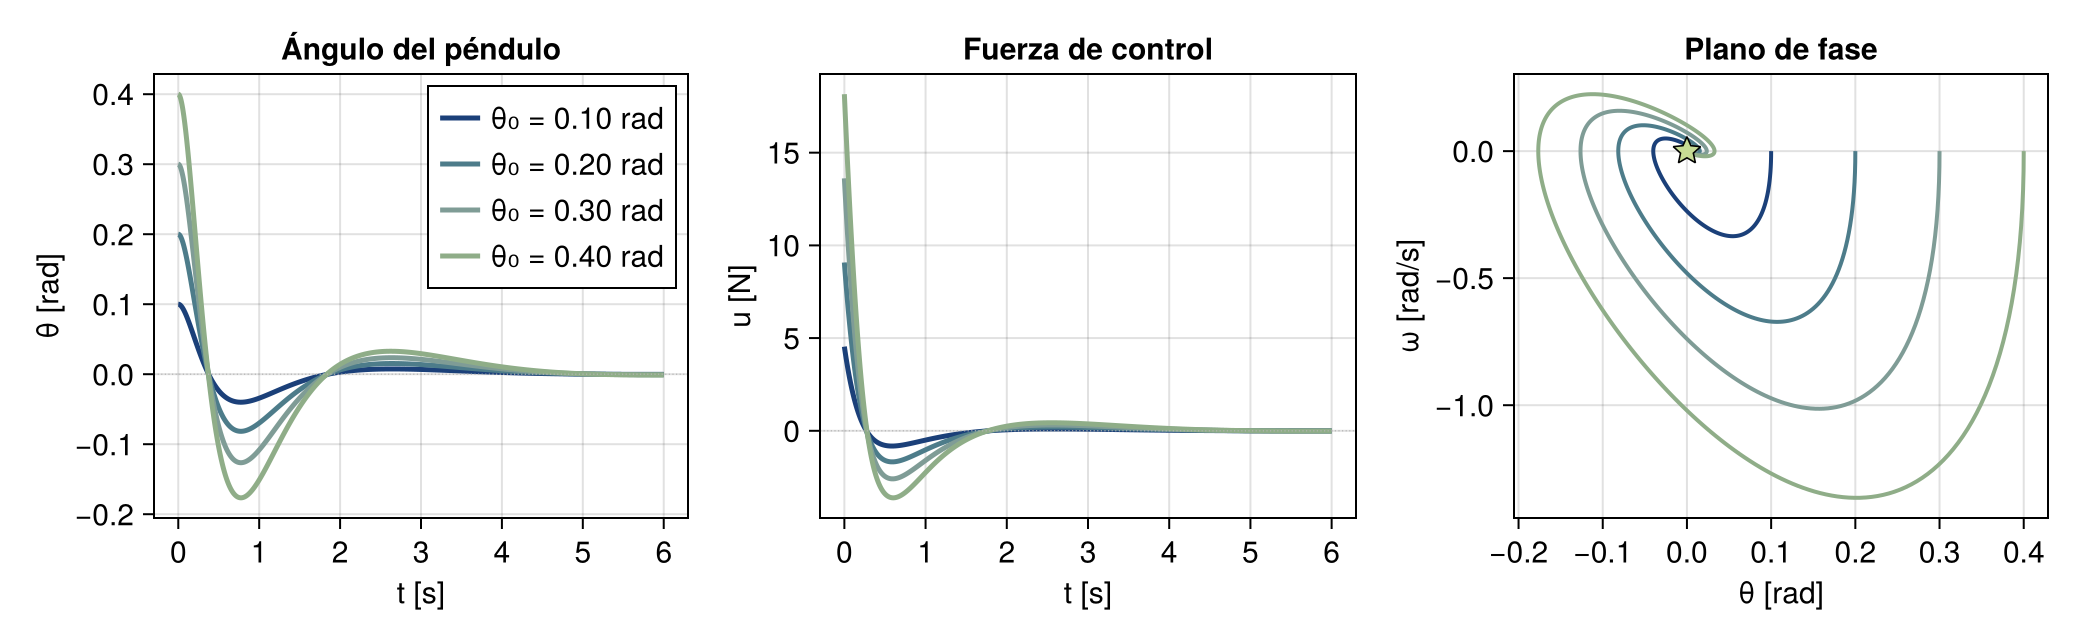
\includegraphics[width=0.98\linewidth]{slides_simple_casos.png}
  \vspace{0.2em}

  \small El controlador LQR, dise\~nado sobre el modelo \emph{lineal},
  estabiliza el modelo no lineal incluso desde $\theta_0=0.40$ rad
  $\approx23^\circ$ ---muy fuera de la vecindad de linealizaci\'on---
  con $t_s$ de $1.30$ a $3.49$ s y $\max|u|$ de $4.5$ a $18.2$ N.
  En el plano de fase, todas las trayectorias convergen al origen.
\end{frame}

\begin{frame}{Respuesta del péndulo doble ($\theta_1=\theta_2=0.1$ rad)}
  \centering
  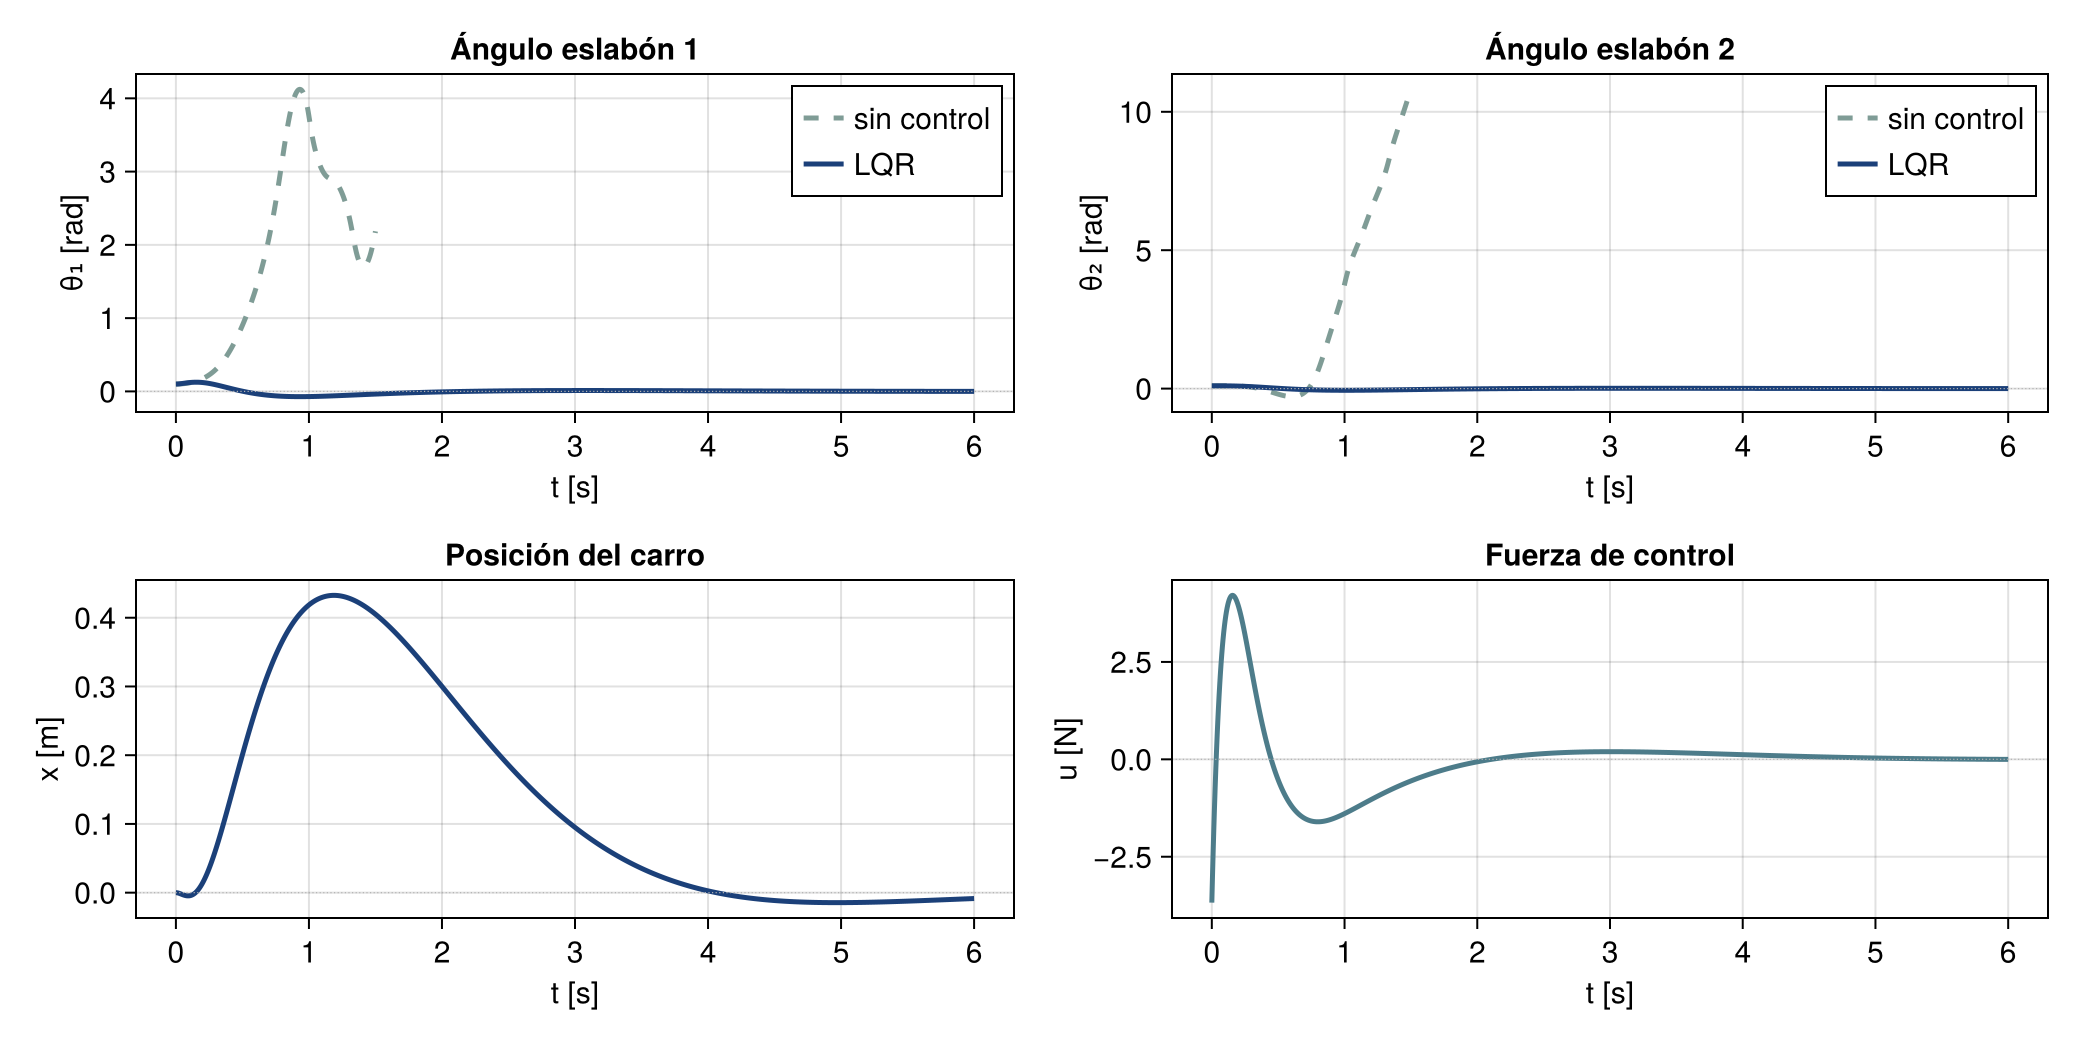
\includegraphics[width=0.72\linewidth]{slides_doble_respuesta.png}
  \vspace{0.15em}

  \small Sin control ambos eslabones caen; con LQR los dos \'angulos se anulan
  en $t_s\approx1.8$ s con $\max|u|=4.2$ N. El costo se traslada a una mayor
  excursi\'on del carro ($0.43$ m frente a $0.33$ m del simple).
\end{frame}

% ============================================================
\section{Conclusiones}
% ============================================================

\begin{frame}{Conclusiones}
  \begin{itemize}
    \item Euler--Lagrange + Taylor llevan la f\'isica no lineal a
          $\dot\xv=A\xv+B\uv$; todo el comportamiento queda cifrado en el
          \'algebra de $A$.
    \item El espectro diagnostica: un modo inestable en el simple, dos en el
          doble; la teor\'ia del polinomio minimal justifica cu\'ando vale la
          diagonalizaci\'on (y el doble \emph{ejercita} un bloque de Jordan
          genuino).
    \item Los criterios de rango de Kalman certifican controlabilidad y
          observabilidad completas: el espectro puede reubicarse y el estado
          reconstruirse.
    \item Ackermann y LQR (Riccati v\'ia hamiltoniana) estabilizan ambas
          configuraciones, \emph{verificado sobre el modelo no lineal} y robusto
          m\'as all\'a de la vecindad lineal.
  \end{itemize}
  \vspace{0.3em}
  \begin{cajaclave}
    \small Un pu\~nado de conceptos ---exponencial matricial, an\'alisis
    espectral, Cayley--Hamilton, teor\'ia del rango y subespacios invariantes---
    constituye el lenguaje natural para modelar, analizar y controlar un sistema
    din\'amico.
  \end{cajaclave}
\end{frame}

\begin{frame}{Referencias}
  \small
  \begin{itemize}
    \item K. Ogata, \emph{Modern Control Engineering}, 5.\textsuperscript{a} ed., Prentice Hall, 2010.
    \item C.-T. Chen, \emph{Linear System Theory and Design}, 3.\textsuperscript{a} ed., Oxford University Press, 1999.
    \item K. Hoffman y R. Kunze, \emph{Linear Algebra}, 2.\textsuperscript{a} ed., Prentice Hall, 1971.
    \item G. Strang, \emph{Introduction to Linear Algebra}, 5.\textsuperscript{a} ed., Wellesley--Cambridge Press, 2016.
    \item M. W. Hirsch, S. Smale y R. L. Devaney, \emph{Differential Equations, Dynamical Systems, and an Introduction to Chaos}, 2.\textsuperscript{a} ed., Elsevier, 2004.
    \item G. H. Golub y C. F. Van Loan, \emph{Matrix Computations}, 4.\textsuperscript{a} ed., Johns Hopkins University Press, 2013.
    \item A. V\'elez, \emph{Notas del curso: C\'alculo de Variaciones}, Universidad Nacional de Colombia, Sede Medell\'in, 2026.
  \end{itemize}
  \vspace{0.4em}
  \footnotesize Informe t\'ecnico, resumen ejecutivo y c\'odigo completo en el
  repositorio del proyecto:
  \href{https://github.com/sauribee/proyecto-pendulos.git}{\textcolor{petroleo}{Enlace}}.
\end{frame}

% ── Cierre ──────────────────────────────────────────────────
\begin{frame}[plain]
\begin{tikzpicture}[remember picture,overlay]
  \fill[marino] (current page.south west) rectangle (current page.north east);
  \franjapaleta{1.15cm}
  \node[anchor=center, text=white, align=center] at (current page.center)
    {\parbox{0.8\paperwidth}{\centering
      {\LARGE\bfseries ¡Gracias!}\\[1.0em]
      {\normalsize Preguntas y discusi\'on}\\[1.6em]
      {\footnotesize\color{black!10}{mabedoyar@unal.edu.co} \quad {cpatinoo@unal.edu.co} \quad \texttt{sauribee@unal.edu.co}}}};
\end{tikzpicture}
\end{frame}

\end{document}
